\documentclass[11pt,a4paper]{article}

\usepackage{../../templates/style}

\begin{document}

\begin{problem}{Tiling}{standard input}{standard output}{1 second}{64 megabytes}

ห้องที่มหาวิทยาลัยขอนแก่นได้มีการปูพื้นกระเบื้องใหม่ในช่วงของการแข่งขันคอมพิวเตอร์โอลิมปิก สอวน โดยเฉพาะ ห้องมีหลายขนาดโดยทุกห้องจะเป็นสี่เหลี่ยมจัตุรัสที่มีขนาด $n \times n$ โดย $n$ เป็นจำนวนเต็ม ซึ่งทุกห้องจะมีมุมห้องด้านบนขวาที่จะไม่ปูกระเบื้อง ทั้งนี้กระเบื้องหนึ่งแผ่นมีขนาด $1 \times 1$ หน่วย



ตัวอย่างเช่น ถ้า $n$ มีขนาดเท่ากับ $2, 3$ และ $4$ ตามลำดับ จะได้การวางกระเบื้องตามลำดับดังแสดงในภาพที่ 1 โดยสีขาวจะเป็นตำแหน่งของกระเบื้อง ส่วนสีดำเป็นส่วนช่องว่างที่ไม่ได้ปู

\begin{figure}[h]
\centering
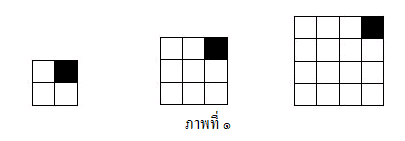
\includegraphics[width=0.7\textwidth]{../latex/img/1015/1015-1.png}
\end{figure}

อย่างไรก็ตามนอกจากรูปห้องจะประหลาดแล้ว กระเบื้องที่สั่งซื้อมาก็ยังประหลาดอีก โดยกระเบื้องจะถูกนำมาติดกันเป็น \textit{“ผืน”} โดยหนึ่งผืนจะมีเพียงสี่แบบซึ่งเป็นการนำกระเบื้องสามแผ่นมาวางติดกัน ดังภาพที่ 2 แม้ว่าเมื่อหมุนแล้วจะดูหน้าตาเหมือนกัน แต่ช่างปูกระเบื้องก็เป็นคนประหลาดอีกที่ไม่ยอมหมุนกระเบื้อง ทำให้ลักษณะของผืนกระเบื้องจะมีลักษณะดังที่เห็นในภาพ

\begin{figure}[h]
\centering
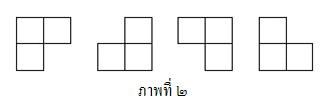
\includegraphics[width=0.6\textwidth]{../latex/img/1015/1015-2.png}
\end{figure}
\newpage
\textbf{ตัวอย่าง}

\begin{figure}[h]
\centering
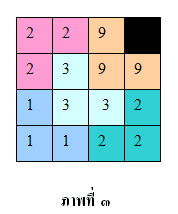
\includegraphics[width=0.3\textwidth]{../latex/img/1015/1015-3.png}
\end{figure}


ภาพที่ 3 แสดงตัวอย่างของการปูผืนกระเบื้อง กระเบื้องทุกแผ่นจะมีหมายเลขเป็นจำนวนเต็มกำกับ แต่ละแผ่นอาจมีหมายเลขที่ซ้ำกันได้ กระเบื้องที่มีหมายเลขเดียวกันและอยู่ติดกันจะถือว่าอยู่บน “ผืน” เดียวกัน

\begin{figure}[h]
\centering
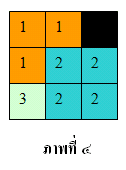
\includegraphics[width=0.2\textwidth]{../latex/img/1015/1015-4.png}
\end{figure}


ภาพที่ 4 แสดงการปูกระเบื้องที่ใช้ผืนกระเบื้องที่ถูกต้อง (ผืนหมายเลข 1) อยู่หนึ่งผืนปะปนอยู่กับผืนกระเบื้องที่ไม่ถูกต้อง (ผืนหมายเลข 2 และ 3)



\underline{\textbf{โจทย์}}  จงเขียนโปรแกรมเพื่อนับจำนวนผืนกระเบื้องที่มีลักษณะถูกต้อง

\InputFile

\textbf{บรรทัดแรก} รับเลขจำนวนเต็มบวก $n$ ซึ่งบอกขนาดของห้อง $(2 \leq n \leq 17)$

\textbf{บรรทัดที่ $2$ ถึง $n+1$} บรรทัดที่ $i+1$ ให้รับรายละเอียดการปูกระเบื้องแถวที่ $i$ โดยแต่ละบรรทัดประกอบด้วยจำนวนเต็ม $n$ ค่าคั่นด้วยช่องว่างหนึ่งช่อง ซึ่งจำนวนเต็ม $k$ $(1 \leq k \leq 9)$ แต่ละตัวคือหมายเลขของกระเบื้อง ทั้งนี้จำนวนเต็ม $0$ แทนมุมห้องที่ไม่ได้ปูกระเบื้อง

\OutputFile

\textbf{มีบรรทัดเดียว} แสดงจำนวนเต็มค่าเดียว ซึ่งแทนจำนวนผืนกระเบื้องที่ถูกต้อง

\Examples

\begin{example}
\exmp{3
1 1 0
1 2 2
3 2 2}{1}%
\exmp{5
3 3 6 6 0
3 5 5 6 8
2 2 5 8 8
2 1 4 4 7
1 1 4 7 7}{8}%
\end{example}


\Source

การแข่งขันคอมพิวเตอร์โอลิมปิก สอวน. ครั้งที่ 3 มหาวิทยาลัยขอนแก่น

\end{problem}

\end{document}